\section{Harun Ar - Rasyid}
\subsection{Teori}
\subsubsection{Apa itu fungsi device manager di windows dan folder /dev di linux}
Fungsi device manager dan folder /dev itu berfungsi untuk mengetahui device apa saja yang telah terinstal di leptop anda serta mengetahui port yang digunakan oleh device tersebut.

\subsubsection{Jelaskan langkah-langkah instalasi driver dari arduino}
\begin{enumerate}
    \item Cara Auto
    \begin{itemize}
        \item Pertama Hubungkan sistem minimum Arduino Uno ke komputer dengan kabel USB type B(kabel Printer)
        \begin{figure}[H]	
            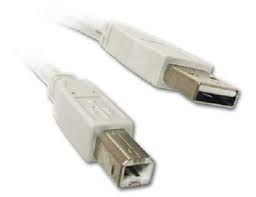
\includegraphics[width=5cm]{figures/5/1174027/teori/1.jpg}
            \centering
            \caption{Membuat file csv}
        \end{figure}

        \item Lalu pada bagian kanan didesktop PC anda, akan muncul popup “Installing device driver software” seperti pada gambar dibawah ini.
        \begin{figure}[H]	
            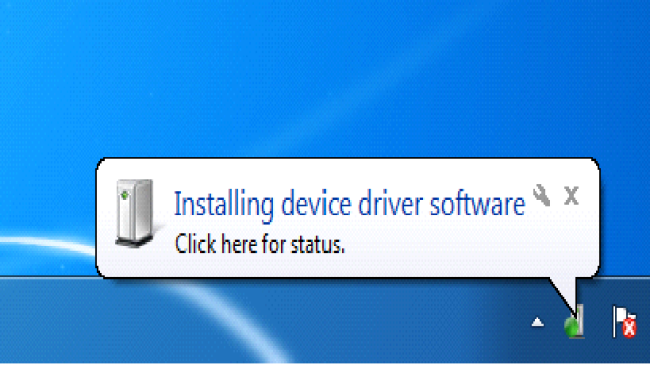
\includegraphics[width=5cm]{figures/5/1174027/teori/2.png}
            \centering
            \caption{Membuat file csv}
        \end{figure}

        \item Tunggu hingga selesai.
        \item Jika sudah selesai anda bisa mengecheck di device manager.
        \begin{figure}[H]	
            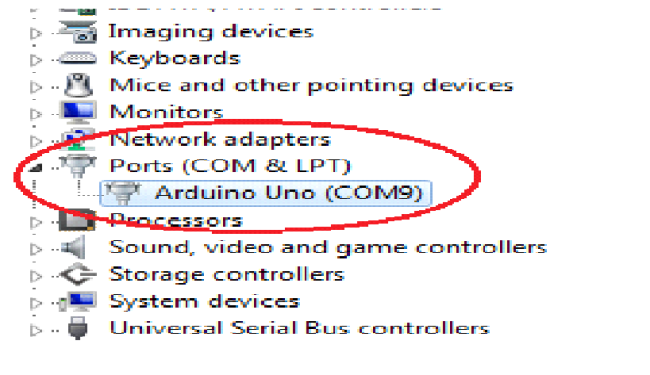
\includegraphics[width=5cm]{figures/5/1174027/teori/11.png}
            \centering
            \caption{Membuat file csv}
        \end{figure}
    \end{itemize}

    \item Cara Manual

    \begin{itemize}
        \item Penginstalan secara manual akan dilakukan jika penginstalan secara auto gagal dilakukan.
        \item Buka Device Manager, caranya pada bagian Search Program and Files lalu ketikkan “device manager”, perhatikan gambar dibawah ini. Pada bagian Control Panel akan muncul Device Manager, klik untuk menjalankan.
            \begin{figure}[H]	
                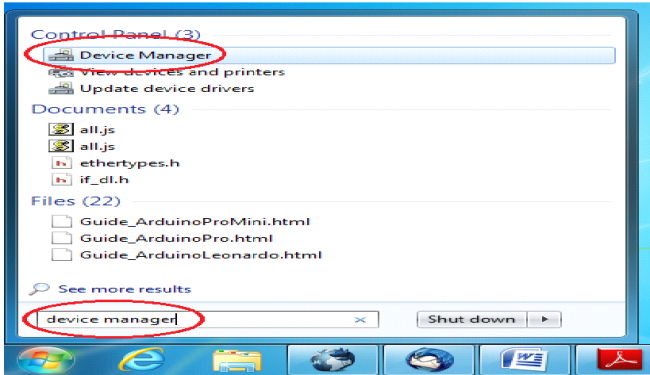
\includegraphics[width=5cm]{figures/5/1174027/teori/4.png}
                \centering
                \caption{Membuat file csv}
            \end{figure}

        \item Cari Unknown device pada bagian Other device, biasanya terdapat tanda seru berwarna kuning, itu disebabkan karena penginstallan tidak berjalan dengan sempurna.
        \begin{figure}[H]	
            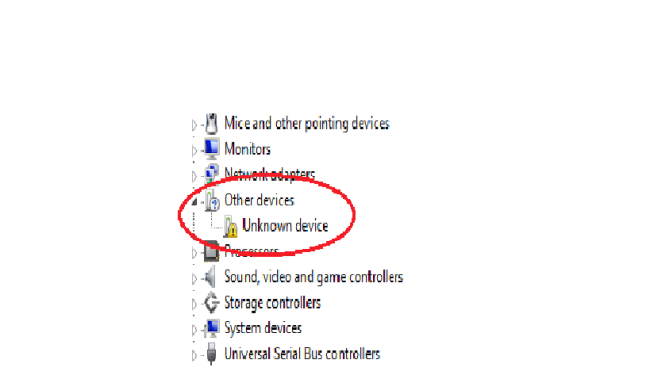
\includegraphics[width=5cm]{figures/5/1174027/teori/5.png}
            \centering
            \caption{Membuat file csv}
        \end{figure}

        \item Klik kanan pada “Unknown device” kemudian pilih Update Driver Software.
        \begin{figure}[H]	
            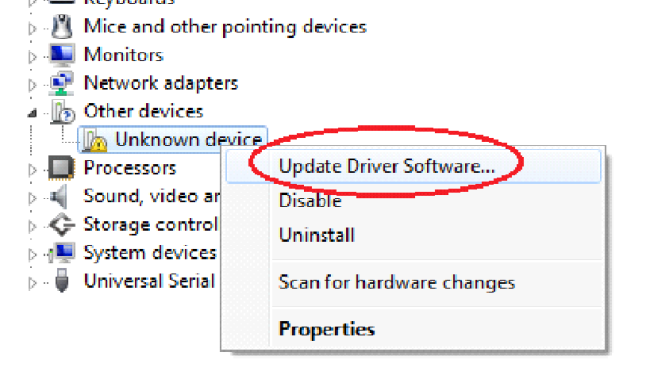
\includegraphics[width=5cm]{figures/5/1174027/teori/6.png}
            \centering
            \caption{Membuat file csv}
        \end{figure}

        \item Pilih Browse my computer for driver software.
        \begin{figure}[H]	
            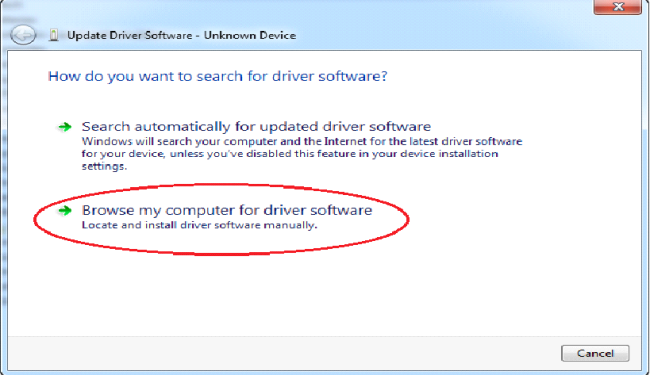
\includegraphics[width=5cm]{figures/5/1174027/teori/7.png}
            \centering
            \caption{Membuat file csv}
        \end{figure}

        \item Arahkan lokasi folder ke folder ..arduino-1.0.5 drivers. Pastikan check-box lalu centang include subfolders. Klik Next untuk melanjutkan instalasi driver.
        \begin{figure}[H]	
            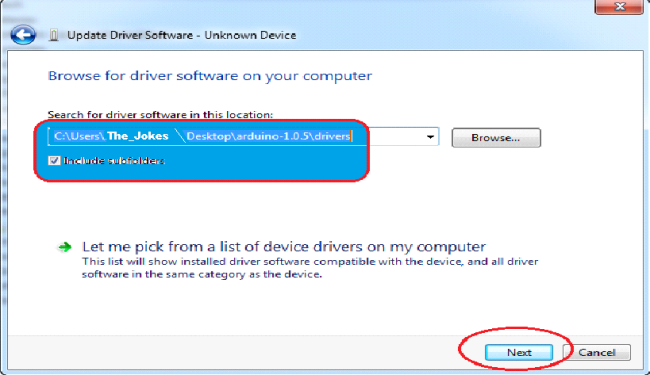
\includegraphics[width=5cm]{figures/5/1174027/teori/8.png}
            \centering
            \caption{Membuat file csv}
        \end{figure}

        \item Kemudian lanjutkan dengan mengklik Install pada tampilan Windows Security.
        \begin{figure}[H]	
            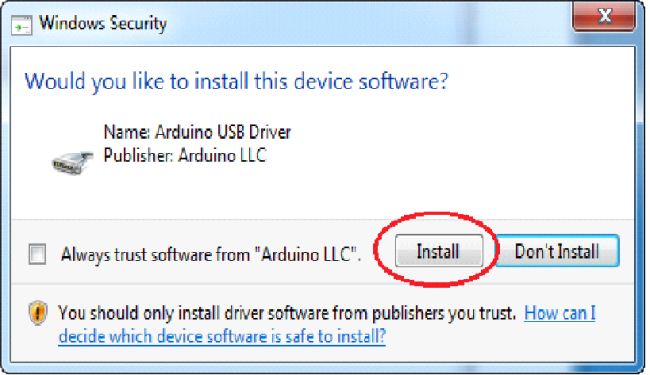
\includegraphics[width=5cm]{figures/5/1174027/teori/9.png}
            \centering
            \caption{Membuat file csv}
        \end{figure}

        \item Jika instalasi driver berhasil maka akan muncul Windows has successfully updated your driver software.
        \begin{figure}[H]	
            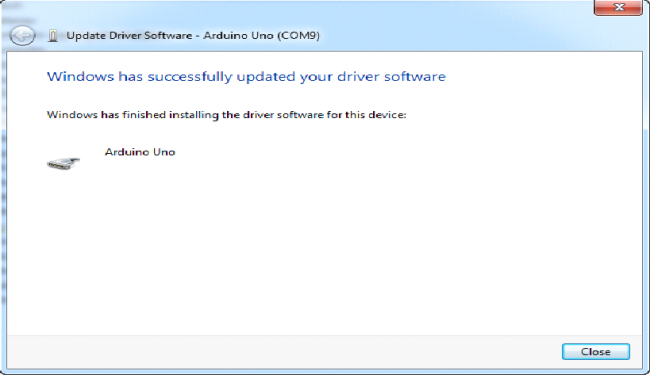
\includegraphics[width=5cm]{figures/5/1174027/teori/10.png}
            \centering
            \caption{Membuat file csv}
        \end{figure}

        \item Perhatikan dan ingat nama COM Arduino Uno, karena nama COM ini yang akan digunakan untuk meng-upload program nantinya.
        \begin{figure}[H]	
            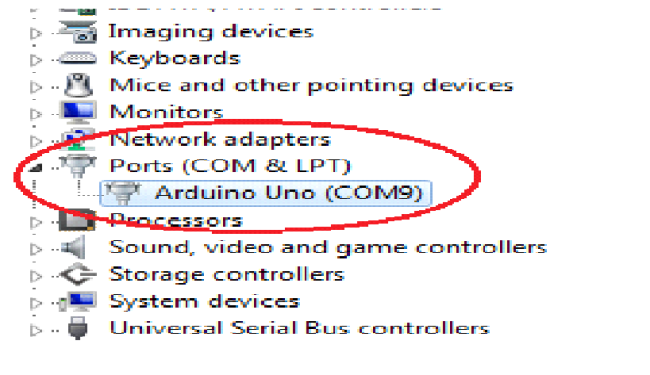
\includegraphics[width=5cm]{figures/5/1174027/teori/11.png}
            \centering
            \caption{Membuat file csv}
        \end{figure}
        \end{itemize}
\end{enumerate}
\subsubsection{Jelaskan bagaimana cara membaca baudrate dan port dari komputer yang sudah terinstall driver}
Untuk baudrate itu bisa dicek melalui arduino IDE, kemudian untuk mengecheck port bisa dilakukan dengan device manager

\subsubsection{Jelaskan sejarah library pyserial}
Modul ini merangkum akses untuk port serial. Ini menyediakan backends untuk Python yang berjalan di Windows, Linux, BSD (mungkin sistem yang mendukung POSIX), Jython dan IronPython (.NET dan Mono). Modul bernama "serial" secara otomatis memilih backend yang sesuai. Antarmuka berbasis kelas yang sama pada semua platform yang didukung.
Akses ke pengaturan port melalui properti Python.
Dukungan untuk berbagai ukuran byte, bit stop, paritas dan kontrol aliran dengan RTS / CTS dan / atau Xon / Xoff.
Bekerja dengan atau tanpa menerima batas waktu.
File seperti API dengan "read" dan "write" ("readline" dll. Juga didukung).
File-file dalam paket ini adalah 100 persen Python murni.
Port diatur untuk transmisi biner. Tidak ada stripping byte NULL, terjemahan CR-LF dll. (Yang berkali-kali diaktifkan untuk POSIX.) Ini membuat modul ini bermanfaat secara universal.
Kompatibel dengan pustaka io (Python 2.6+)

\subsubsection{Jelaskan fungsi-fungsi apa saja yang dipakai dari library pyserial}


Serial – fungsi ini untuk membuka port serial
Write(data) – untuk menulis data lewat port serial
Readline() – untuk membaca string dari port serial
Read(size) – untuk membaca jumlah byte dari port serial
Close() – ini untuk menutup port serial 

\subsubsection{Jelaskan kenapa butuh perulangan dan tidak butuh perulangan dalam membaca serial}


Perualangan dalam bahasa pemrograman berfungsi menyuruh komputer melakukan sesuatu secara berulang-ulang. Terdapat dua jenis perualangan dalam bahasa pemrograman python, yaitu perulangan dengan for dan while.
Perulangan for disebut counted loop (perulangan yang terhitung), sementara perulangan while disebut uncounted loop (perulangan yang tak terhitung). Perbedaannya adalah perulangan for biasanya digunakan untuk mengulangi kode yang sudah diketahui banyak perulangannya. Sementara while untuk perulangan yang memiliki syarat dan tidak tentu berapa banyak perulangannya.
Perulangan diperlukan agar dapat membaca data secara berulang kali sehingga data yang muncul lebih dari satu.  Sedangkan apabila tidak memakai perulangan maka data akan terbaca satu kali saja.

\subsubsection{Jelaskan bagaimana cara membuat fungsi yang mengunakan pyserial}


Berikut merupakan contoh penggunaan fungsi yang menggunakan pyserial
\lstinputlisting[firstline=8, lastline=15]{src/5/1174027/teori/T1174027.py}

\subsubsection{Scan Plagiarisme}
\begin{figure}[H]	
    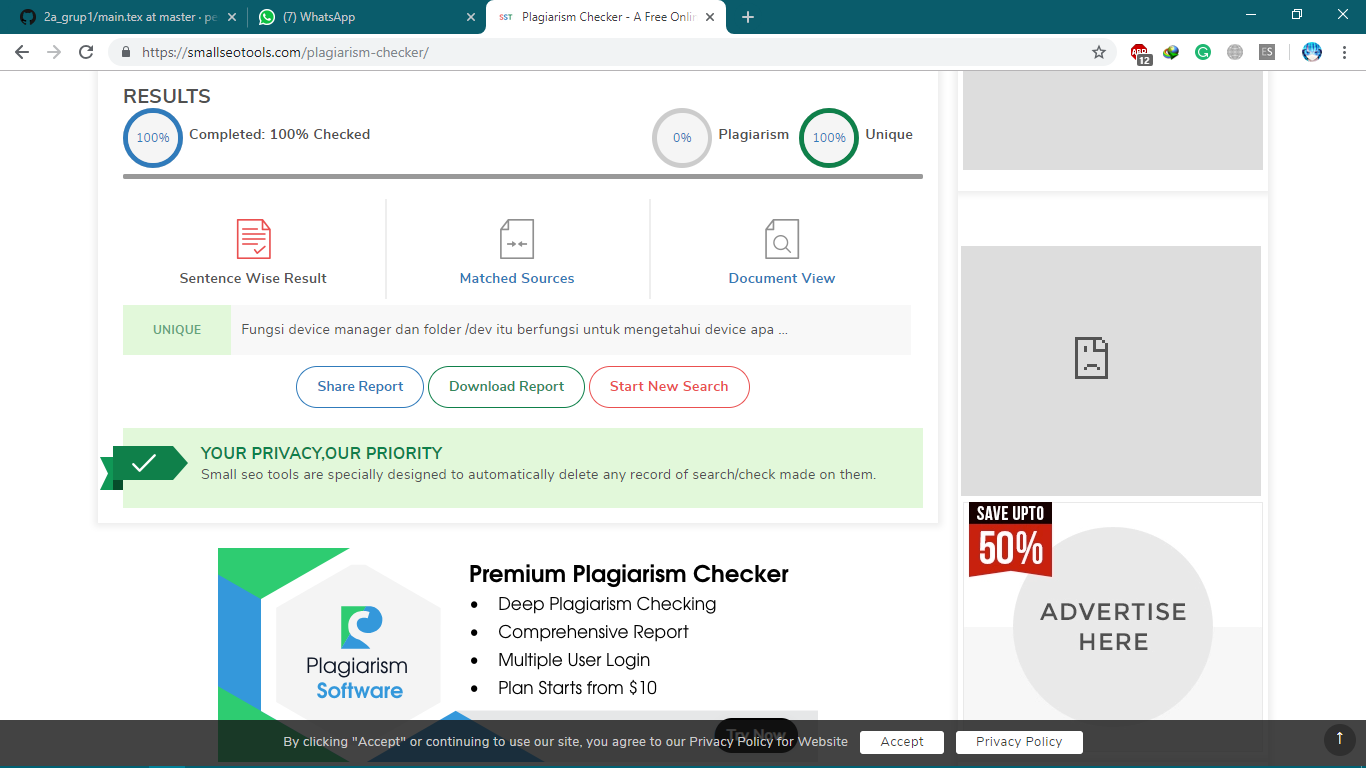
\includegraphics[width=5cm]{figures/5/1174027/teori/nopla.png}
    \centering
    \caption{Membuat file csv}
\end{figure}

\subsection{Praktek}
\subsubsection{Buatlah fungsi (file terpisah/library dengan nama NPM realtime.py) untuk mendapatkan data langsung dari arduino}
\lstinputlisting[firstline=8, lastline=14]{src/5/1174027/praktek/1174027_realtime.py}

\subsubsection{Buatlah fungsi (file terpisah/library dengan nama NPM save.py) untuk mendapatkan data langsung dari arduino dengan looping}
\lstinputlisting[firstline=8, lastline=15]{src/5/1174027/praktek/1174027_save.py}

\subsubsection{Buatlah fungsi (file terpisah/library dengan nama NPM realtime.py) untuk mendapatkan data dari arduino dan langsung ditulis kedalam file csv}
\lstinputlisting[firstline=16, lastline=29]{src/5/1174027/praktek/1174027_realtime.py}

\subsubsection{Buatlah fungsi (file terpisah/library dengan nama NPM csv.py) untuk membaca file csv hasil arduino dan mengembalikan ke fungsi}
\lstinputlisting[firstline=8, lastline=16]{src/5/1174027/praktek/1174027_csv.py}

\subsubsection{Penanganan Error}
Untuk kali ini saya menemukan Type Error, yaitu error yang menampilkan jika type data na berbeda berusaha disatukan.
\lstinputlisting[firstline=8, lastline=17]{src/5/1174027/praktek/1174027.py}